% =====================================================================
%  Lern- und Erklärskript zu Versuch 9: Anlauf- und Bremsverfahren
%  Persönliche Lernhilfe (nicht abzugeben)
%  Übersetzen: pdflatex erklaerung.tex (2x)
% =====================================================================
\documentclass[11pt,a4paper]{article}
\usepackage[utf8]{inputenc}
\usepackage[T1]{fontenc}
\usepackage[ngerman]{babel}
\usepackage{lmodern}
\usepackage{microtype}
\usepackage[a4paper,left=2.3cm,right=2.3cm,top=2.5cm,bottom=2.5cm]{geometry}
\usepackage{amsmath,amssymb}
\usepackage[locale=DE,per-mode=symbol]{siunitx}
\usepackage{graphicx}
\usepackage{booktabs}
\usepackage{float}
\usepackage{enumitem}
\setlist{itemsep=2pt,topsep=4pt}
\usepackage{xcolor}
\usepackage[colorlinks=true,linkcolor=black,urlcolor=blue!50!black]{hyperref}
\usepackage[most]{tcolorbox}
\usepackage{fancyhdr}

\graphicspath{{../bericht/abbildungen/}}
% automatisch erzeugt von auswertung/auswertung.py
\newcommand{\WJStahl}{0{,}3711}
\newcommand{\WJAlu}{0{,}1277}
\newcommand{\WJVorb}{0{,}3745}
\newcommand{\WdtBsp}{42{,}6}
\newcommand{\WtHDA}{1{,}20}
\newcommand{\WtHDB}{1{,}29}
\newcommand{\WtHDC}{1{,}40}
\newcommand{\WtHYA}{3{,}62}
\newcommand{\WtHYB}{3{,}92}
\newcommand{\WtHYC}{4{,}24}
\newcommand{\WdirektIeins}{50{,}66}
\newcommand{\WdirektUnull}{405}
\newcommand{\WdirektUeins}{388}
\newcommand{\WdirektPeins}{17896}
\newcommand{\WdirektQeins}{56162}
\newcommand{\Wdirektnend}{1499}
\newcommand{\WdirektIend}{4{,}58}
\newcommand{\WdirektPend}{1747}
\newcommand{\WdirektQend}{5175}
\newcommand{\Wdirekttneunacht}{1{,}14}
\newcommand{\Wdirektteinsvierfuenfnull}{1{,}10}
\newcommand{\WdirektE}{14509}
\newcommand{\WdirektdU}{4{,}3}
\newcommand{\WdirektIfak}{11{,}0}
\newcommand{\WdirektIN}{7{,}6}
\newcommand{\WfruehIeins}{15{,}51}
\newcommand{\WfruehUnull}{405}
\newcommand{\WfruehUeins}{400}
\newcommand{\WfruehPeins}{6685}
\newcommand{\WfruehQeins}{17788}
\newcommand{\Wfruehnend}{1497}
\newcommand{\WfruehIend}{4{,}59}
\newcommand{\WfruehPend}{1760}
\newcommand{\WfruehQend}{5173}
\newcommand{\Wfruehtneunacht}{2{,}65}
\newcommand{\Wfruehteinsvierfuenfnull}{2{,}62}
\newcommand{\WfruehE}{15389}
\newcommand{\WfruehdU}{1{,}2}
\newcommand{\WfruehIfak}{3{,}4}
\newcommand{\WfruehIN}{2{,}3}
\newcommand{\Wfruehtum}{1{,}91}
\newcommand{\Wfruehnum}{724}
\newcommand{\Wfruehpause}{0{,}16}
\newcommand{\WfruehIzwei}{45{,}91}
\newcommand{\WfruehUzwei}{384}
\newcommand{\WfruehPzwei}{20422}
\newcommand{\WfruehdUzwei}{5{,}1}
\newcommand{\WrichtigIeins}{15{,}51}
\newcommand{\WrichtigUnull}{405}
\newcommand{\WrichtigUeins}{400}
\newcommand{\WrichtigPeins}{5635}
\newcommand{\WrichtigQeins}{17779}
\newcommand{\Wrichtignend}{1497}
\newcommand{\WrichtigIend}{4{,}57}
\newcommand{\WrichtigPend}{1755}
\newcommand{\WrichtigQend}{5162}
\newcommand{\Wrichtigtneunacht}{3{,}86}
\newcommand{\Wrichtigteinsvierfuenfnull}{3{,}82}
\newcommand{\WrichtigE}{15754}
\newcommand{\WrichtigdU}{1{,}3}
\newcommand{\WrichtigIfak}{3{,}4}
\newcommand{\WrichtigIN}{2{,}3}
\newcommand{\Wrichtigtum}{3{,}60}
\newcommand{\Wrichtignum}{1443}
\newcommand{\Wrichtigpause}{0{,}14}
\newcommand{\WrichtigIzwei}{42{,}25}
\newcommand{\WrichtigUzwei}{402}
\newcommand{\WrichtigPzwei}{11284}
\newcommand{\WrichtigdUzwei}{0{,}9}
\newcommand{\WfalschIeins}{15{,}71}
\newcommand{\WfalschUnull}{405}
\newcommand{\WfalschUeins}{400}
\newcommand{\WfalschPeins}{5622}
\newcommand{\WfalschQeins}{18202}
\newcommand{\Wfalschnend}{1498}
\newcommand{\WfalschIend}{4{,}58}
\newcommand{\WfalschPend}{1781}
\newcommand{\WfalschQend}{5172}
\newcommand{\Wfalschtneunacht}{3{,}90}
\newcommand{\Wfalschteinsvierfuenfnull}{3{,}59}
\newcommand{\WfalschE}{15842}
\newcommand{\WfalschdU}{1{,}3}
\newcommand{\WfalschIfak}{3{,}4}
\newcommand{\WfalschIN}{2{,}4}
\newcommand{\Wfalschtum}{3{,}62}
\newcommand{\Wfalschnum}{1453}
\newcommand{\Wfalschpause}{0{,}15}
\newcommand{\WfalschIzwei}{50{,}91}
\newcommand{\WfalschUzwei}{401}
\newcommand{\WfalschPzwei}{19180}
\newcommand{\WfalschdUzwei}{1{,}0}
\newcommand{\WtHYum}{3{,}87}
\newcommand{\WdirektMBmittel}{52{,}7}
\newcommand{\WfruehMBmittel}{14{,}8}
\newcommand{\WrichtigMBmittel}{15{,}8}
\newcommand{\WfalschMBmittel}{15{,}9}
\newcommand{\WMkennDmittel}{48{,}8}
\newcommand{\WMkennYmittel}{16{,}1}
\newcommand{\WEkin}{2268}
\newcommand{\Wfedernnull}{1801}
\newcommand{\WfedertB}{0{,}88}
\newcommand{\Wfederts}{0{,}12}
\newcommand{\WfederMmit}{31{,}7}
\newcommand{\WfederMmax}{32{,}0}
\newcommand{\WfederUzkmax}{583}
\newcommand{\WfederErb}{0}
\newcommand{\Wfederverz}{2047}
\newcommand{\Wfedernullnnull}{1801}
\newcommand{\WfedernulltB}{0{,}90}
\newcommand{\Wfedernullts}{0{,}12}
\newcommand{\WfedernullMmit}{30{,}8}
\newcommand{\WfedernullMmax}{31{,}3}
\newcommand{\WfedernullUzkmax}{583}
\newcommand{\WfedernullErb}{0}
\newcommand{\Wfedernullverz}{1996}
\newcommand{\WdclnI}{1773}
\newcommand{\WdclIdcB}{14{,}1}
\newcommand{\WdclIeffB}{9{,}4}
\newcommand{\WdcltI}{1{,}03}
\newcommand{\WdcltnachI}{5{,}17}
\newcommand{\Wdclnnull}{1801}
\newcommand{\WdcltB}{6{,}20}
\newcommand{\Wdclts}{0{,}40}
\newcommand{\WdclMmit}{4{,}6}
\newcommand{\WdclMmax}{21{,}4}
\newcommand{\WdclUzkmax}{595}
\newcommand{\WdclErb}{0}
\newcommand{\Wdclverz}{290}
\newcommand{\WdcmnI}{1774}
\newcommand{\WdcmIdcB}{20{,}5}
\newcommand{\WdcmIeffB}{13{,}7}
\newcommand{\WdcmtI}{1{,}02}
\newcommand{\WdcmtnachI}{2{,}43}
\newcommand{\Wdcmnnull}{1801}
\newcommand{\WdcmtB}{3{,}45}
\newcommand{\Wdcmts}{0{,}41}
\newcommand{\WdcmMmit}{9{,}7}
\newcommand{\WdcmMmax}{33{,}9}
\newcommand{\WdcmUzkmax}{596}
\newcommand{\WdcmErb}{0}
\newcommand{\Wdcmverz}{521}
\newcommand{\WdcsnI}{1774}
\newcommand{\WdcsIdcB}{32{,}8}
\newcommand{\WdcsIeffB}{21{,}9}
\newcommand{\WdcstI}{1{,}03}
\newcommand{\WdcstnachI}{0{,}95}
\newcommand{\Wdcsnnull}{1801}
\newcommand{\WdcstB}{1{,}98}
\newcommand{\Wdcsts}{0{,}42}
\newcommand{\WdcsMmit}{25{,}5}
\newcommand{\WdcsMmax}{57{,}5}
\newcommand{\WdcsUzkmax}{596}
\newcommand{\WdcsErb}{0}
\newcommand{\Wdcsverz}{929}
\newcommand{\Wgenohnennull}{1801}
\newcommand{\WgenohnetB}{8{,}49}
\newcommand{\Wgenohnets}{0{,}09}
\newcommand{\WgenohneMmit}{2{,}9}
\newcommand{\WgenohneMmax}{19{,}6}
\newcommand{\WgenohneUzkmax}{815}
\newcommand{\WgenohneErb}{0}
\newcommand{\Wgenohneverz}{211}
\newcommand{\Wgenlnnull}{1801}
\newcommand{\WgenltB}{10{,}12}
\newcommand{\Wgenlts}{0{,}14}
\newcommand{\WgenlMmit}{2{,}4}
\newcommand{\WgenlMmax}{2{,}8}
\newcommand{\WgenlUzkmax}{724}
\newcommand{\WgenlErb}{512}
\newcommand{\Wgenlverz}{177}
\newcommand{\Wgenmnnull}{1801}
\newcommand{\WgenmtB}{5{,}13}
\newcommand{\Wgenmts}{0{,}10}
\newcommand{\WgenmMmit}{4{,}8}
\newcommand{\WgenmMmax}{5{,}8}
\newcommand{\WgenmUzkmax}{724}
\newcommand{\WgenmErb}{1365}
\newcommand{\Wgenmverz}{349}
\newcommand{\Wgensnnull}{1801}
\newcommand{\WgenstB}{0{,}87}
\newcommand{\Wgensts}{0{,}06}
\newcommand{\WgensMmit}{29{,}6}
\newcommand{\WgensMmax}{39{,}2}
\newcommand{\WgensUzkmax}{723}
\newcommand{\WgensErb}{1821}
\newcommand{\Wgensverz}{2061}
\newcommand{\WRb}{28}
\newcommand{\WPRbmax}{7760}
\newcommand{\WgensErbAnteil}{80}


\newtcolorbox{merke}{colback=green!5,colframe=green!45!black,fonttitle=\bfseries,
  title={Merke},boxrule=0.6pt,arc=1mm}
\newtcolorbox{einfach}{colback=yellow!7,colframe=orange!70!black,fonttitle=\bfseries,
  title={Einfach erklärt},boxrule=0.6pt,arc=1mm}
\newtcolorbox{frage}[1]{colback=blue!4,colframe=blue!50!black,fonttitle=\bfseries\small,
  title={#1},boxrule=0.6pt,arc=1mm}
\newtcolorbox{achtung}{colback=red!4,colframe=red!60!black,fonttitle=\bfseries,
  title={Achtung / Prüfe selbst},boxrule=0.6pt,arc=1mm}

\pagestyle{fancy}\fancyhf{}
\fancyhead[L]{Lernskript V9}\fancyhead[R]{Anlauf- und Bremsverfahren}
\fancyfoot[C]{\thepage}

\begin{document}
\sloppy
\begin{center}
{\LARGE\bfseries Lernskript zu Versuch 9}\\[4pt]
{\Large Anlauf- und Bremsverfahren der Asynchronmaschine}\\[6pt]
{\normalsize Alle Punkte des Versuchs Schritt für Schritt erklärt -- zum Verstehen, Lernen und für das Testat}
\end{center}
\tableofcontents
\newpage

% =====================================================================
\section{Worum geht es im Versuch? (Der rote Faden)}
% =====================================================================
Der Versuch hat zwei Teile:
\begin{enumerate}
\item \textbf{Anlauf:} Wie schaltet man einen Asynchronmotor ein, ohne das Netz zu stark
  zu belasten? Verglichen werden der \emph{direkte Dreieckanlauf} und der
  \emph{Stern-Dreieck-Anlauf}. Vorher berechnet man, wie lange der Hochlauf dauert.
\item \textbf{Bremsen:} Wie bekommt man einen drehenden Motor mit Schwungscheibe schnell
  zum Stehen? Verglichen werden \emph{Federkraftbremse}, \emph{DC-Bremse} und
  \emph{generatorisches Bremsen} (mit und ohne Bremswiderstand).
\end{enumerate}
Die eine Formel, die alles zusammenhält, ist die \textbf{Bewegungsgleichung}:
\[
  J\cdot\frac{\mathrm d\omega}{\mathrm dt} = M_\mathrm{Motor} - M_\mathrm{Last}.
\]
\begin{einfach}
Ein Drehmoment beschleunigt oder bremst eine Drehmasse, so wie eine Kraft ein Auto
beschleunigt oder bremst ($F = m\cdot a$). Hier gilt $M = J\cdot\alpha$:
\begin{itemize}
\item $J$ ist die \glqq Masse beim Drehen\grqq{} (Massenträgheitsmoment, in \si{kg.m^2}),
\item $\alpha = \mathrm d\omega/\mathrm dt$ ist die Winkelbeschleunigung.
\end{itemize}
Mit dieser Formel kannst du in \emph{beide Richtungen} rechnen:
\begin{itemize}
\item Moment bekannt $\Rightarrow$ Zeit ausrechnen (Vorbereitung, Hochlaufzeit).
\item Drehzahlverlauf gemessen $\Rightarrow$ Moment ausrechnen (Auswertung).
\end{itemize}
\end{einfach}

% =====================================================================
\section{Grundlagen, die du verstehen musst}
% =====================================================================
\subsection{Warum ist der Anlaufstrom so groß?}
Ein stehender Asynchronmotor ist wie ein \textbf{Transformator mit kurzgeschlossener
Sekundärseite}: Der Läuferkäfig ist ein Kurzschlussring. Im Stillstand (Schlupf
$s = 1$) dreht sich das Ständerfeld mit voller Geschwindigkeit am Läufer vorbei. Es wird
eine große Spannung induziert, und es fließt ein großer Strom. Begrenzt wird er nur durch
die kleine Kurzschlussimpedanz.

\textbf{Schlupf:} $s = \dfrac{n_s - n}{n_s}$, mit $n_s = \dfrac{f}{p}$ (synchrone
Drehzahl). Bei \SI{50}{Hz} und $p=2$ gilt $n_s = \SI{1500}{\per\minute}$.
\begin{itemize}
\item Stillstand: $s = 1$, großer Strom.
\item Nenndrehzahl \SI{1420}{\per\minute}: $s \approx 0{,}05$, kleiner Strom.
\end{itemize}

\textbf{Gemessen:} Direktanlauf \SI{\WdirektIeins}{A}, das ist das \WdirektIN-fache des
Nennstroms von \SI{6,65}{A}. Das liegt genau im Lehrbuchbereich (5- bis 8-fach).

\subsection{Warum bricht die Netzspannung ein?}
Das Netz (Transformator und Kabel) hat einen Innenwiderstand $Z_k = R_k + \mathrm jX_k$.
Fließt ein großer Strom, fällt daran Spannung ab, und beim Motor kommt weniger an.

\textbf{Warum gerade beim Anlauf so stark?}
\begin{itemize}
\item Der Anlaufstrom ist fast reiner Blindstrom (gemessen $\cos\varphi \approx 0{,}3$).
\item Beim Transformator ist $X_k$ viel größer als $R_k$.
\item Der Spannungsabfall $\mathrm jX_k\cdot I$ liegt dann fast parallel zur
  Netzspannung und zieht sie direkt nach unten.
\end{itemize}
Das ist das \textbf{Kapp'sche Dreieck}:
$\Delta U \approx I\,(R_k\cos\varphi + X_k\sin\varphi)$.
Bei $\sin\varphi \approx 1$ wirkt der volle Wert $X_k\cdot I$.

\subsection{Stern und Dreieck -- die Faktoren \texorpdfstring{$\sqrt3$}{Wurzel 3} und 3}
\begin{center}
\begin{tabular}{@{}lcc@{}}
\toprule
& Stern (Y) & Dreieck ($\Delta$)\\
\midrule
Spannung am Wicklungsstrang & $400/\sqrt3 = \SI{230}{V}$ & \SI{400}{V}\\
Strangstrom & $\frac{1}{\sqrt3}\cdot I_{\mathrm{Str},\Delta}$ & $I_{\mathrm{Str},\Delta}$\\
Netzstrom (Leiterstrom) & $\frac13\cdot I_{\mathrm{Netz},\Delta}$ & $I_{\mathrm{Netz},\Delta} = \sqrt3\, I_{\mathrm{Str},\Delta}$\\
Drehmoment ($\sim U^2$) & $\frac13\cdot M_\Delta$ & $M_\Delta$\\
\bottomrule
\end{tabular}
\end{center}
\textbf{Herleitung des Faktors 3 beim Netzstrom:}
\begin{itemize}
\item Im Stern ist die Strangspannung um $\sqrt3$ kleiner, also auch der Strangstrom.
\item Im Dreieck ist der Netzstrom zusätzlich um $\sqrt3$ größer als der Strangstrom.
\item Zusammen: $\sqrt3\cdot\sqrt3 = 3$.
\end{itemize}
\textbf{Gemessen:} $\WdirektIeins/\WrichtigIeins \approx 3{,}3$, passt also gut.

\textbf{Warum $M \sim U^2$?} Der Fluss ist proportional zu $U$ und der Läuferstrom
ebenfalls proportional zu $U$. Das Moment ist Fluss mal Strom, also proportional zu $U^2$.

\begin{merke}
Stern-Dreieck senkt Strom \emph{und} Moment auf ein Drittel. Deshalb funktioniert es nur,
wenn die Last beim Anlauf klein ist (Lüfter, Pumpen, Schwungmasse ohne Last). Für
Förderbänder oder Hubwerke unter Last reicht ein Drittel des Moments oft nicht.
\end{merke}

\subsection{Die Momentkennlinie \texorpdfstring{$M(n)$}{M(n)}}
Wichtige Punkte (siehe Abb.~\ref{fig:kenn}):
\begin{itemize}
\item \textbf{Anzugsmoment} bei $n=0$: hier \SI{46}{Nm}.
\item \textbf{Sattelmoment}, ein kleiner Einbruch bei ca.\ \SI{200}{\per\minute}. Er entsteht
      durch Oberwellen und ist typisch für Käfigläufer.
\item \textbf{Kippmoment}, das Maximum: ca.\ \SI{56}{Nm} bei \SI{1000}{\per\minute}.
\item Danach fällt das Moment steil ab und ist bei $n_s = \SI{1500}{\per\minute}$ null.
      Ohne Schlupf wird nichts induziert, also entsteht kein Moment.
\end{itemize}
\begin{figure}[H]\centering
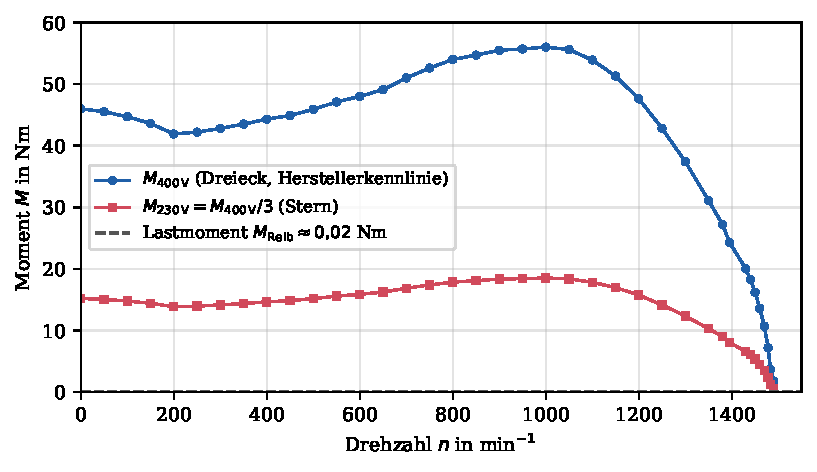
\includegraphics[width=0.8\textwidth]{v_kennlinie}
\caption{Momentkennlinie (aus der Anleitung abgelesen) und Sternkennlinie (ein Drittel)}
\label{fig:kenn}
\end{figure}

\subsection{Das Massenträgheitsmoment \texorpdfstring{$J$}{J}}
Für eine Vollscheibe gilt $J = \frac12 m r^2$, mit dem Radius $r = d/2 = \SI{0,15}{m}$.
\begin{itemize}
\item Stahlscheibe (Anlauf): $J = 0{,}5\cdot 32{,}99\cdot 0{,}15^2 = \SI{\WJStahl}{kg.m^2}$.
\item Aluscheibe (Bremsen): $J = 0{,}5\cdot 11{,}35\cdot 0{,}15^2 = \SI{\WJAlu}{kg.m^2}$.
\item Die Anleitung nennt \SI{0,3745}{kg.m^2}. Das ist etwas mehr als die Stahlscheibe allein,
      wahrscheinlich ist das Trägheitsmoment des Motorläufers mit eingerechnet.
\end{itemize}

% =====================================================================
\section{Vorbereitung: Hochlaufzeit berechnen -- Schritt für Schritt}
% =====================================================================
\textbf{Idee:} Man teilt den Drehzahlbereich in kleine Stücke (z.\,B.\ je
\SI{50}{\per\minute}). In jedem Stück nimmt man das Moment als konstant an und rechnet
aus, wie lange das Stück dauert. Am Ende werden alle Zeiten addiert. Das nennt man
\textbf{numerische Integration}.

\textbf{Herleitung der Formel:}
\begin{align*}
J\,\frac{\Delta\omega}{\Delta t} &= M
\quad\Rightarrow\quad \Delta t = \frac{J\,\Delta\omega}{M},
\qquad \Delta\omega = 2\pi\,\Delta n \;(\Delta n \text{ in } \si{\per\second})\\
\Rightarrow\quad \Delta t &= \frac{2\pi\,J\,\Delta n}{M}.
\end{align*}

\textbf{Beispiel} für den ersten Schritt von 0 auf \SI{50}{\per\minute} im Dreieck:
\begin{enumerate}
\item Drehzahlschritt in \si{\per\second} umrechnen: $\Delta n = 50/60 = \SI{0,833}{\per\second}$.
\item Einsetzen: $\Delta t = 2\pi\cdot 0{,}3745\cdot 0{,}833 / 46 = \SI{0,0426}{s}
      \approx \SI{42}{ms}$. Das ist genau der Wert aus der Anleitung.
\item Im Stern ist das Moment nur $46/3 = \SI{15,3}{Nm}$, der Schritt dauert also
      dreimal so lange: ca.\ \SI{128}{ms}.
\end{enumerate}

\textbf{So gehst du in Excel vor} (oder wie im Python-Skript):
\begin{enumerate}
\item Spalte A: Drehzahl $n$, Spalte B: Moment $M_{400}$ (abgelesen).
\item Spalte C: $M_{230} = B/3$.
\item Spalte D: mittleres Moment im Intervall $(B_i + B_{i+1})/2$, minus \SI{0,02}{Nm} Reibung.
\item Spalte E: $\Delta t = 2\pi\cdot J\cdot (A_{i+1}-A_i)/60 / D$.
\item Spalte F: aufsummierte Zeit $t$.
\item Diagramm $n$ über $t$ zeichnen -- \textbf{nicht normiert}, also mit echten
      Sekunden und \si{\per\minute}, so wie es die Anleitung verlangt.
\end{enumerate}

\textbf{Ergebnis:}
\begin{itemize}
\item Dreieck: \SI{\WtHDB}{s} bis \SI{1450}{\per\minute}.
\item Stern: \SI{\WtHYB}{s} bis \SI{1450}{\per\minute}, genau dreimal so lang.
\end{itemize}
Daraus folgt: Im Stern sollte man nach ca.\ \SIrange{3,6}{3,9}{s} umschalten.

\begin{achtung}
\begin{itemize}
\item Kurz vor \SI{1500}{\per\minute} geht $M \to 0$, und $\Delta t$ wird sehr groß. Darum
      rechnet man nur bis z.\,B.\ \SI{1450}{} oder \SI{1480}{\per\minute}. Das solltest du
      begründen können.
\item Ich habe die Kennlinie aus dem Bild in der Anleitung abgelesen. Wenn ihr in StudIP
      die CSV-Datei mit der Kennlinie habt, nimm deren Werte. Die Zeiten ändern sich dann leicht.
\end{itemize}
\end{achtung}

\begin{figure}[H]\centering
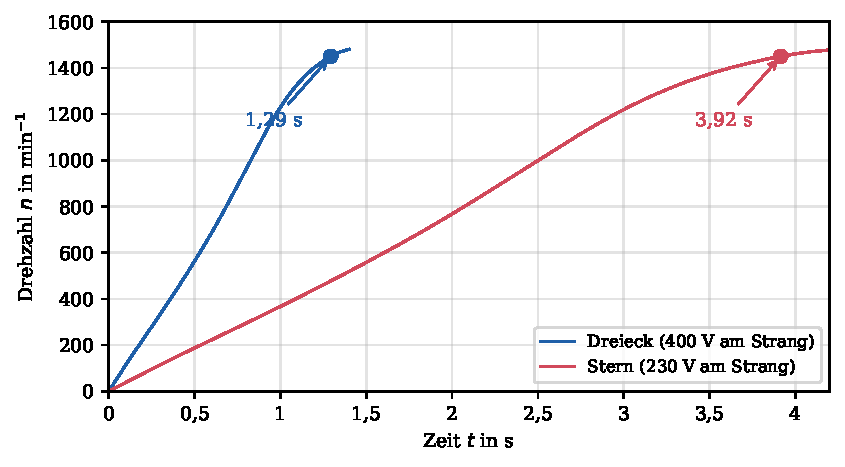
\includegraphics[width=0.8\textwidth]{v_hochlauf}
\caption{Berechneter Hochlauf}
\end{figure}

% =====================================================================
\section{Anlaufversuche: Was zeigen die Diagramme?}
% =====================================================================
\textbf{Lesehilfe:} Jedes Anlaufdiagramm hat vier Teile übereinander:
\begin{enumerate}
\item Drehzahl $n$,
\item Strom $I$,
\item Spannung $U$,
\item Wirkleistung $P$ und Blindleistung $Q$.
\end{enumerate}
Grau markiert ist die Umschaltpause, in der der Motor kurz stromlos ist.

\subsection{Direkter Dreieckanlauf (Datei \texttt{Stern-Dreieck\_direkt.csv})}
\begin{figure}[H]\centering
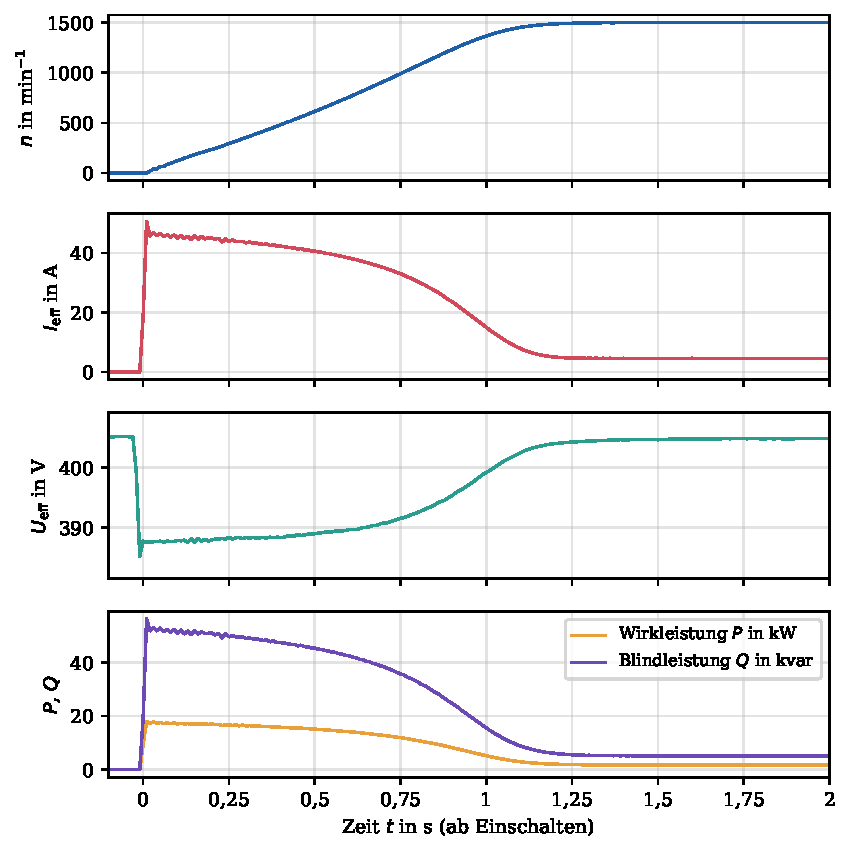
\includegraphics[width=0.72\textwidth]{a_direkt}
\end{figure}
\textbf{Ablauf:}
\begin{enumerate}
\item Einschalten: Der Strom springt auf ca.\ \SI{50}{A}, die Spannung fällt von
      \SI{405}{V} auf \SI{388}{V} (\SI{\WdirektdU}{\percent}).
\item Der Strom bleibt lange hoch. Bis zum Kippschlupf ist die Impedanz klein.
\item Ab ca.\ \SI{1000}{\per\minute} (Kippmoment) fällt der Strom schnell auf den
      Leerlaufstrom von \SI{4,6}{A}, und die Spannung erholt sich.
\item Nach \SI{\Wdirekttneunacht}{s} ist der Hochlauf fertig.
\end{enumerate}

\textbf{Leistungen:}
\begin{itemize}
\item $Q \approx 3\cdot P$, also $\cos\varphi \approx 0{,}3$: Der Anlaufstrom ist vor allem Blindstrom.
\item Im Leerlauf ist $P \approx \SI{1,75}{kW}$. Das sind Eisen-, Reibungs- und Kupferverluste
      im Leerlauf. Der Motor hat keine Last.
\end{itemize}

\subsection{Stern-Dreieck zu früh umgeschaltet}
\begin{figure}[H]\centering
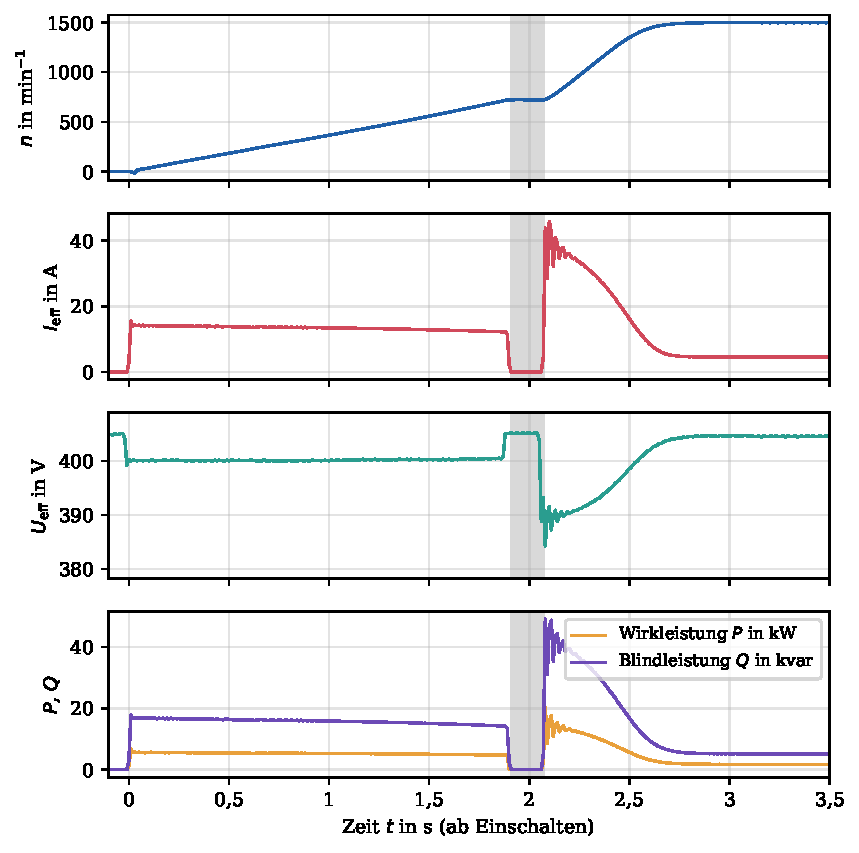
\includegraphics[width=0.72\textwidth]{a_frueh}
\end{figure}
\textbf{Ablauf:}
\begin{enumerate}
\item Im Stern ist der Strom nur ca.\ \SI{15}{A}, ein Drittel. Die Spannung fällt kaum.
\item Die Maschine beschleunigt dreimal langsamer.
\item Umgeschaltet wird schon bei \SI{\Wfruehnum}{\per\minute}. Das ist noch weit weg von
      der Nenndrehzahl, der Schlupf ist noch groß.
\item Im Dreieck fließt deshalb wieder fast der volle Anlaufstrom: \SI{\WfruehIzwei}{A}.
      Die Spannung fällt sogar auf \SI{\WfruehUzwei}{V}.
\end{enumerate}
\textbf{Fazit:} Das Netz bekommt trotzdem einen großen Stromstoß. Der Stern-Dreieck-Anlauf
hat fast nichts gebracht.
\begin{achtung}
Laut Anleitung sollte die Umschaltzeit \SI{0,5}{s} sein. In den Messdaten wird aber erst
nach ca.\ \SI{1,9}{s} umgeschaltet. Vielleicht wurde am Versuchstag ein anderer Wert
eingestellt. Prüfe das in deinen Notizen. Im Bericht steht der Wert, der in den Daten
gemessen wurde.
\end{achtung}

\subsection{Stern-Dreieck richtig umgeschaltet}
\begin{figure}[H]\centering
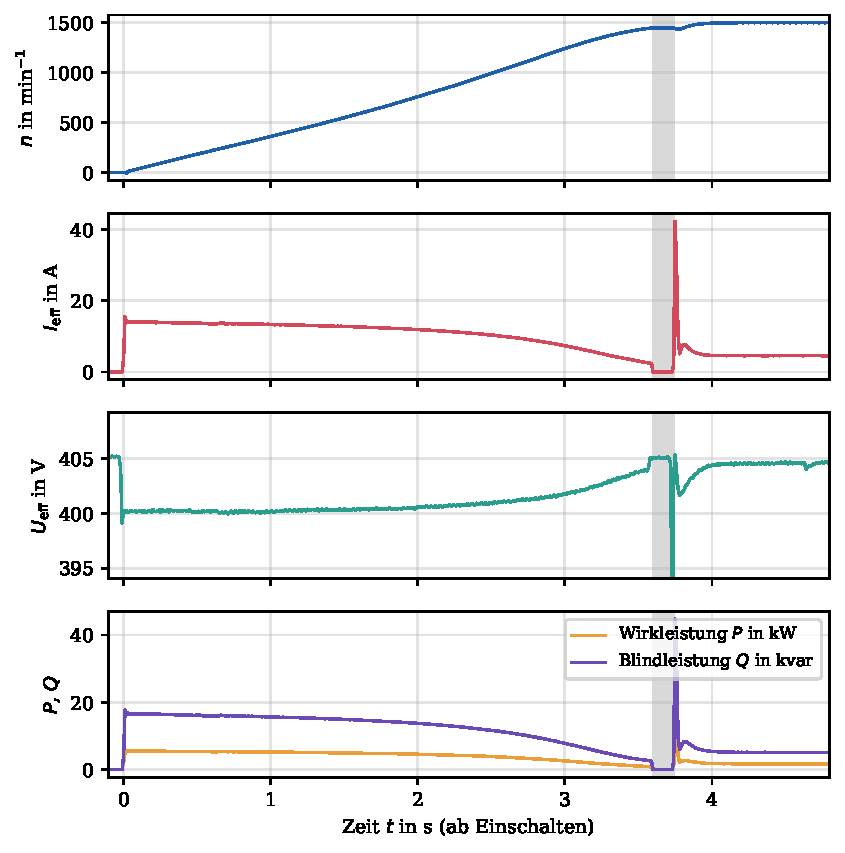
\includegraphics[width=0.72\textwidth]{a_richtig}
\end{figure}
\textbf{Ablauf:}
\begin{enumerate}
\item Umgeschaltet wird bei \SI{\Wrichtignum}{\per\minute}, nach \SI{\Wrichtigtum}{s}.
      Das passt zur Rechnung.
\item Der Strom war vorher schon auf ca.\ \SI{2,5}{A} gefallen.
\item Beim Umschalten gibt es nur eine sehr kurze Spitze (ca.\ \SI{20}{ms}).
\end{enumerate}
\textbf{Woher kommt diese Spitze überhaupt?} Der Läufer ist während der kurzen Pause
noch magnetisiert und erzeugt eine eigene Spannung, die \emph{Restspannung}. Beim
Zuschalten passen Netzspannung und Restspannung nicht genau zusammen. Es entsteht ein
kurzer Ausgleichsstrom.

\subsection{Stern-Dreieck falsch verdrahtet}
\begin{figure}[H]\centering
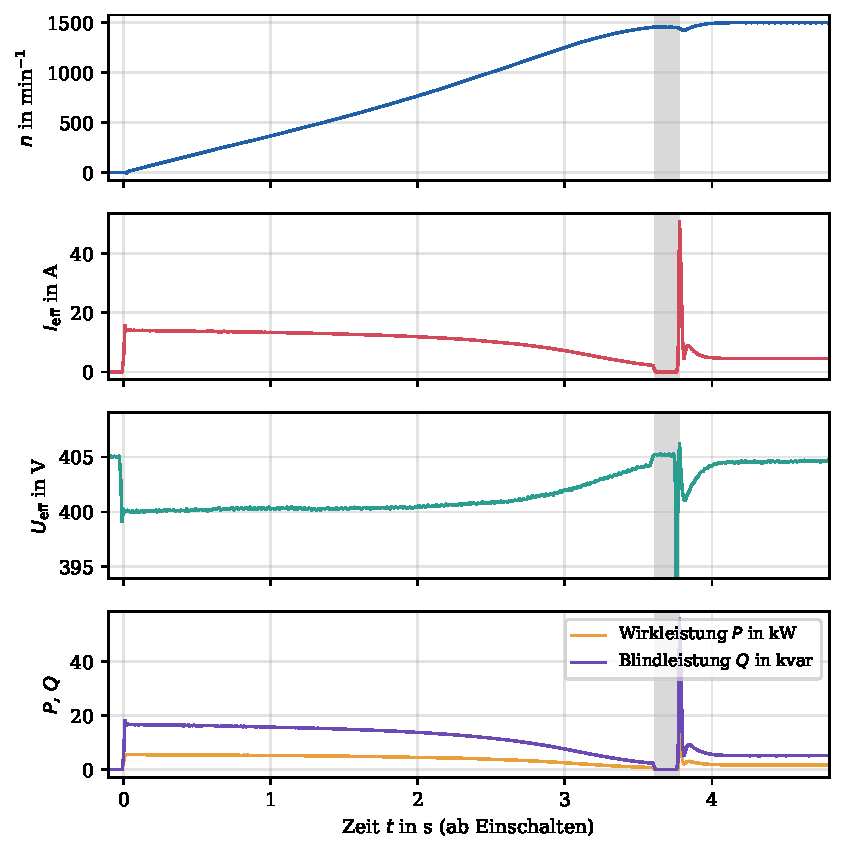
\includegraphics[width=0.72\textwidth]{a_falsch}
\end{figure}
\textbf{Unterschied zu richtig:} Gleiche Umschaltdrehzahl, aber
\begin{itemize}
\item die Stromspitze ist größer (\SI{\WfalschIzwei}{A} statt \SI{\WrichtigIzwei}{A}),
\item die Wirkleistungsspitze ist fast doppelt so hoch,
\item die Drehzahl bricht kurz um ca.\ \SI{30}{\per\minute} ein.
\end{itemize}
\begin{einfach}
\begin{itemize}
\item Beim Umschalten von Stern auf Dreieck dreht sich die Spannung an jedem Strang
      um \SI{30}{\degree}.
\item Ob sie \SI{30}{\degree} vor oder zurück springt, hängt davon ab, wie die Wicklungsenden
      U2, V2, W2 an L1, L2, L3 angeschlossen sind.
\item Bei richtiger Verdrahtung passt die neue Netzspannung gut zur Restspannung des
      Läufers. Es gibt nur einen kleinen Stoß.
\item Bei falscher Verdrahtung ist der Winkel zwischen beiden größer. Es entsteht ein
      größerer Ausgleichsstrom, und für einen Moment bremst er sogar
      (daher der Drehzahleinbruch).
\end{itemize}
\end{einfach}
\begin{achtung}
Diese Erklärung ist die übliche Begründung. Was genau am Versuchstag falsch verdrahtet war,
weißt du nur aus deinen Notizen bzw.\ vom Betreuer. Frag nach, falls unklar.
\end{achtung}

\subsection{Beschleunigungsmoment aus der Messung}
\textbf{Vorgehen:}
\begin{enumerate}
\item Die Drehzahl nach der Zeit ableiten: $\mathrm dn/\mathrm dt$.
\item Mit $J$ und $2\pi$ multiplizieren: $M_B = J\cdot 2\pi\cdot \mathrm dn/\mathrm dt$.
\end{enumerate}
Weil die gemessene Drehzahl rauscht (Messwerte springen um $\pm\SI{1}{\per\minute}$),
muss man vorher glätten. Ich habe einen \emph{Savitzky-Golay-Filter} benutzt. Der legt
stückweise eine Parabel durch die Messpunkte.

\textbf{Excel-Variante:} Differenzenquotient $(n_{i+5}-n_{i-5})/(t_{i+5}-t_{i-5})$ über
mehrere Punkte bilden. Das glättet ebenfalls.
\begin{figure}[H]\centering
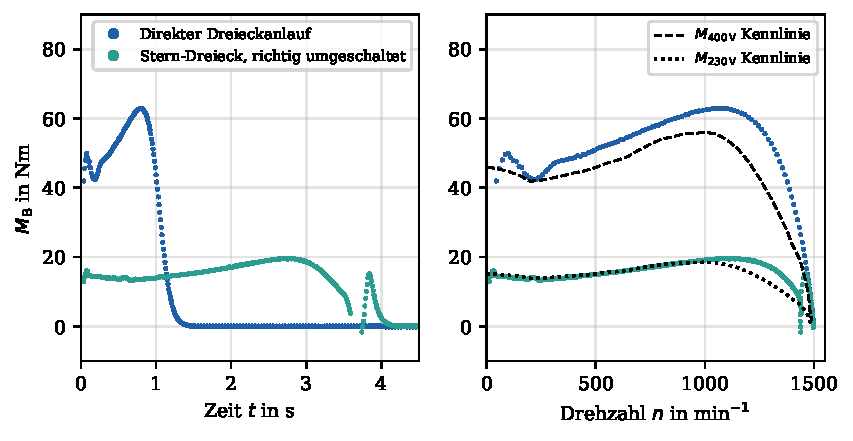
\includegraphics[width=0.9\textwidth]{a_moment}
\end{figure}
\textbf{Ergebnis:}
\begin{itemize}
\item Die Form der Kennlinie ist in der Messung wiederzuerkennen: Sattel, Kipppunkt, Abfall.
\item Im Stern stimmen Messung und Rechnung fast genau überein.
\item Im Dreieck ist das gemessene Moment ca.\ \SI{8}{\percent} größer als die Kennlinie.
      Darum ist die gemessene Hochlaufzeit kürzer als die berechnete
      (\SI{\Wdirektteinsvierfuenfnull}{s} statt \SI{\WtHDB}{s}).
\end{itemize}

\begin{merke}
Gründe, warum Messung und Rechnung abweichen:
\begin{itemize}
\item Die Herstellerkennlinie hat Toleranzen.
\item Die Spannung war \SI{405}{V} statt \SI{400}{V}. Wegen $M \sim U^2$ gibt das
      $+\SI{2,5}{\percent}$ Moment.
\item Die Kennlinie wurde aus einem Bild abgelesen.
\item Der $J$-Wert der Anleitung ist etwas größer.
\item Wo der Hochlauf „fertig“ ist, lässt sich nicht genau festlegen.
\end{itemize}
\end{merke}

\subsection{Energie -- eine schöne Zusatzerkenntnis}
\begin{itemize}
\item In der Schwungscheibe stecken am Ende $E = \frac12 J\omega^2 \approx \SI{4,6}{kJ}$.
\item Aus dem Netz wurden aber ca.\ \SIrange{14,5}{15,8}{kJ} aufgenommen.
\item \textbf{Grund:} Beim Hochlauf einer ASM ohne Last wird im Läufer genauso viel Energie
      verheizt, wie in der Schwungmasse gespeichert wird. Dazu kommen Ständer- und
      Eisenverluste.
\item Stern-Dreieck spart also \emph{keine Energie}. Es verteilt den Strom nur auf eine
      längere Zeit und vermeidet die hohen Spitzen.
\end{itemize}

% =====================================================================
\section{Bremsversuche: Was zeigen die Diagramme?}
% =====================================================================
\textbf{Ausgangslage:}
\begin{itemize}
\item Motor am Frequenzumrichter (FU), Drehzahl ca.\ \SI{1800}{\per\minute} (\SI{60}{Hz}),
      Aluscheibe.
\item $t=0$ ist der Bremsbefehl.
\item Energie in der Scheibe: $E_\mathrm{kin} = \frac12\cdot0{,}1277\cdot(2\pi\cdot30)^2
      \approx \SI{2270}{J}$.
\item Bremsmoment: $M_\mathrm{Br} = -J\cdot 2\pi\cdot\mathrm dn/\mathrm dt$.
\end{itemize}

\subsection{Der Frequenzumrichter in 4 Blöcken}
\begin{enumerate}
\item \textbf{Gleichrichter} (Dioden): macht aus Netzwechselspannung Gleichspannung.
  Er kann nur Energie \emph{aufnehmen}, aber \emph{nicht ins Netz zurückgeben}.
\item \textbf{Zwischenkreis} (Kondensator): ca.\ $\sqrt2\cdot\SI{400}{V}\approx\SI{565}{V}$,
  gemessen \SI{580}{V}.
\item \textbf{Brems-Chopper} mit Bremswiderstand: ein Transistor, der bei zu hoher
  Zwischenkreisspannung den Widerstand zuschaltet.
\item \textbf{Wechselrichter} (IGBTs): erzeugt Drehstrom mit beliebiger Frequenz.
\end{enumerate}
\begin{merke}
Das Wichtigste für alle Bremsfragen: Der Diodengleichrichter ist eine Einbahnstraße.
Die Bremsenergie kann nicht zurück ins Netz. Sie muss in Wärme umgewandelt werden: im
Motor (DC-Bremse), im Bremswiderstand oder in der Reibbremse.
\end{merke}

\subsection{Übersicht}
\begin{figure}[H]\centering
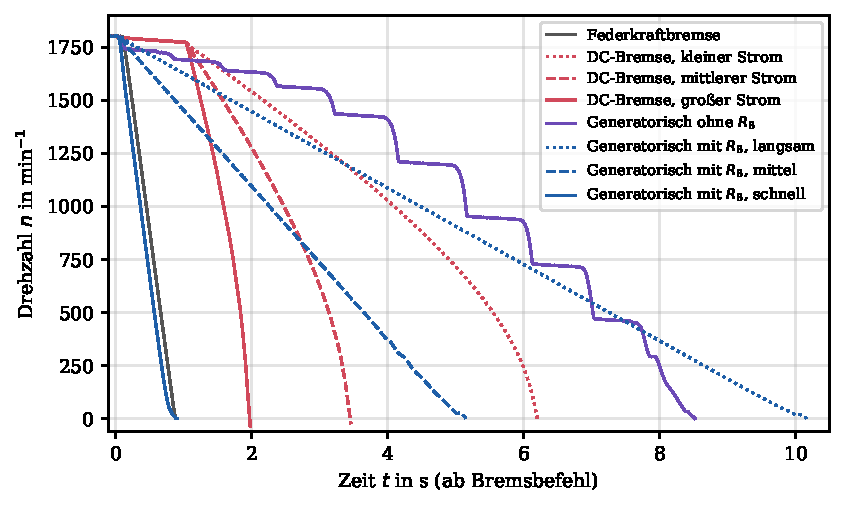
\includegraphics[width=0.85\textwidth]{b_vergleich_n}
\end{figure}

\subsection{Federkraftbremse}
\textbf{Funktionsweise:}
\begin{itemize}
\item Eine Feder drückt die Bremsbeläge zusammen.
\item Ein Elektromagnet hält die Bremse offen (\glqq gelüftet\grqq).
\item Strom weg $\Rightarrow$ Magnet lässt los $\Rightarrow$ die Feder bremst.
\end{itemize}
\textbf{Messung:}
\begin{itemize}
\item ca.\ \SI{\Wfederts}{s} Verzögerung (Einfallzeit: das Magnetfeld muss erst abklingen),
\item dann sinkt die Drehzahl \textbf{linear}, das Moment ist also konstant: ca.\ \SI{\WfederMmit}{Nm},
\item Stillstand nach \SI{\WfedertB}{s}.
\end{itemize}
\textbf{Warum ist das Moment konstant?} Trockene Reibung (Coulomb) hängt nicht von der
Geschwindigkeit ab: Reibkraft $=\mu\cdot$ Federkraft.

\subsection{DC-Bremse (Gleichstrombremsung)}
\textbf{Funktionsweise:}
\begin{itemize}
\item Der FU schickt Gleichstrom durch die Ständerwicklung. Es entsteht ein \emph{stehendes} Magnetfeld.
\item Der drehende Läufer schneidet dieses Feld. Es wird Strom induziert, und es entsteht ein
      Bremsmoment, wie bei einer Wirbelstrombremse.
\end{itemize}
\textbf{Messung:}
\begin{itemize}
\item Zuerst ca.\ \SI{1}{s} lang nichts: Der FU wartet, bis die Restspannung des Motors
      abgeklungen ist (Entmagnetisierungszeit). Sonst gäbe es einen Kurzschlussstrom.
\item Dann wird mit \SI{\WdclIdcB}{A}, \SI{\WdcmIdcB}{A} bzw.\ \SI{\WdcsIdcB}{A} gebremst.
\item Die Bremszeit sinkt dabei von \SI{\WdcltnachI}{s} über \SI{\WdcmtnachI}{s} auf \SI{\WdcstnachI}{s}.
\end{itemize}
\begin{figure}[H]\centering
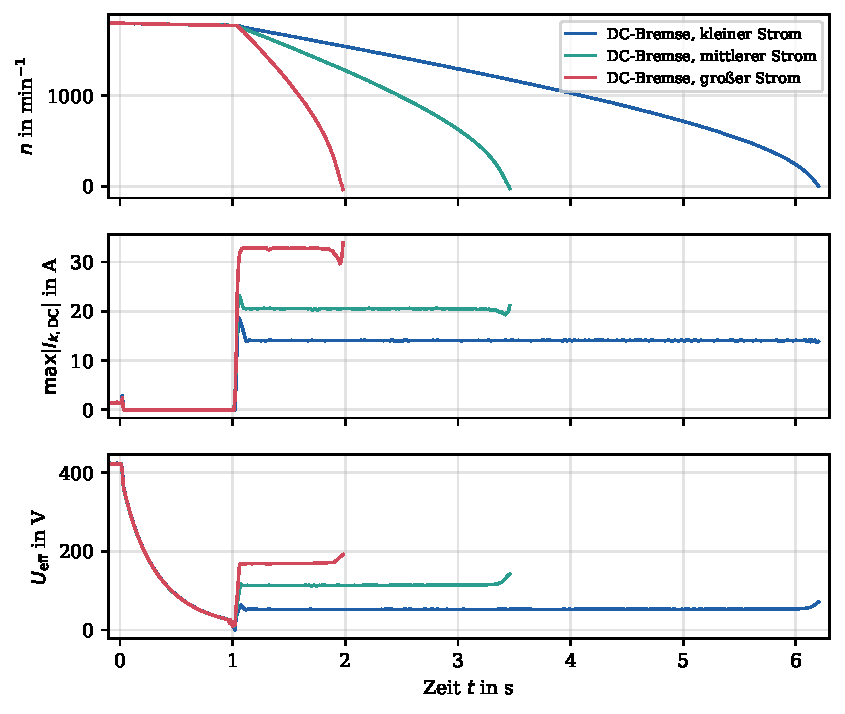
\includegraphics[width=0.72\textwidth]{b_dc}
\end{figure}
\textbf{Drei Dinge, die du erklären können musst:}
\begin{enumerate}
\item \textbf{Moment $\sim I^2$:} Das Feld ist $\sim I$, der induzierte Läuferstrom auch
  $\sim I$, also ist das Moment $\sim I^2$. Gemessen: Strom $\times1{,}45 \Rightarrow$ Moment
  $\times2{,}1$, Strom $\times2{,}33 \Rightarrow$ Moment $\times5{,}5$. Passt!
\item \textbf{Das Moment wird zum Ende hin größer} (die Kurve wird steiler): Bei hoher
  Drehzahl ist die Läuferfrequenz hoch. Dann ist der Läufer stark induktiv, und der Strom
  liegt \glqq falsch\grqq{} zum Feld. Bei kleiner Drehzahl passt es besser. Das Maximum
  liegt deshalb kurz vor dem Stillstand. Es ist wie die Motorkennlinie, nur gespiegelt.
\item \textbf{Kein Haltemoment:} Bei $n=0$ wird nichts mehr induziert, also gibt es kein Moment.
  Eine hängende Last (Kran) würde langsam absinken. Außerdem wird die gesamte Energie im
  \emph{Motor} verheizt, er wird heiß.
\end{enumerate}

\subsection{Generatorisch ohne Bremswiderstand}
\textbf{Funktionsweise:} Der FU senkt die Frequenz. Die Maschine dreht dann schneller als
das Feld ($s<0$) und wird zum Generator. Die Energie fließt in den Zwischenkreis.

\textbf{Messung und Erklärung:}
\begin{itemize}
\item $U_\mathrm{ZK}$ steigt von \SI{580}{V} auf bis zu \SI{\WgenohneUzkmax}{V}.
\item Bei Überspannung schaltet der FU die Pulse ab. Der Strom ist dann null, und der
      Motor trudelt nur aus.
\item Wenn $U_\mathrm{ZK}$ wieder gesunken ist, folgt ein kurzer Bremsimpuls, und das
      Spiel wiederholt sich.
\item Ergebnis: Die Drehzahl fällt in Treppenstufen, Stillstand erst nach \SI{\WgenohnetB}{s}.
\end{itemize}
\begin{figure}[H]\centering
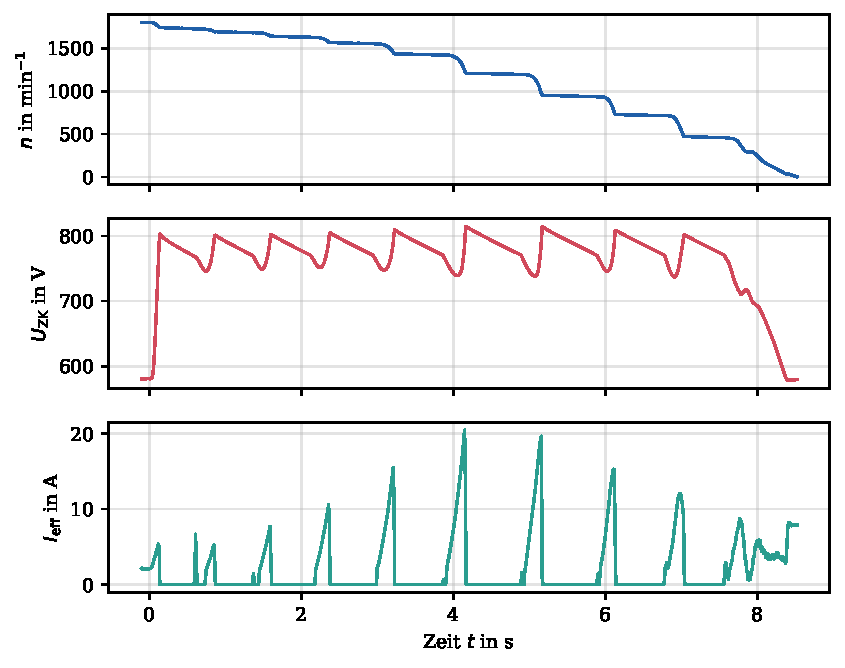
\includegraphics[width=0.72\textwidth]{b_gen0}
\end{figure}

\subsection{Generatorisch mit Bremswiderstand}
\textbf{Messung:}
\begin{itemize}
\item Der Chopper begrenzt $U_\mathrm{ZK}$ auf ca.\ \SI{720}{V}.
\item Der Motor folgt exakt der Rampe: Die Drehzahl sinkt linear, das Moment ist konstant.
\item Bremszeiten: langsam \SI{\WgenltB}{s}, mittel \SI{\WgenmtB}{s}, schnell \SI{\WgenstB}{s}.
\item Schnell: Der Widerstand nimmt bis \SI{7,8}{kW} auf. Insgesamt gehen ca.\ \SI{\WgensErb}{J}
      hinein, das sind \SI{\WgensErbAnteil}{\percent} der kinetischen Energie. Der Rest sind
      Verluste in Motor und Umrichter.
\item Bei der langsamen Rampe schaltet der Chopper kaum, weil die Verluste in Motor und FU
      die kleine Bremsleistung schon fast schaffen.
\end{itemize}

\textbf{Bremswiderstand abschätzen:} Der Chopper schaltet den Strom pulsförmig.
\begin{itemize}
\item Einschaltdauer: $D = (I_\mathrm{mittel}/I_\mathrm{eff})^2$.
\item Strom im eingeschalteten Zustand: $I_\mathrm{ein} = I_\mathrm{mittel}/D$.
\item Widerstand: $R = U_\mathrm{ZK}/I_\mathrm{ein} \approx \SI{\WRb}{\ohm}$.
\end{itemize}
\begin{figure}[H]\centering
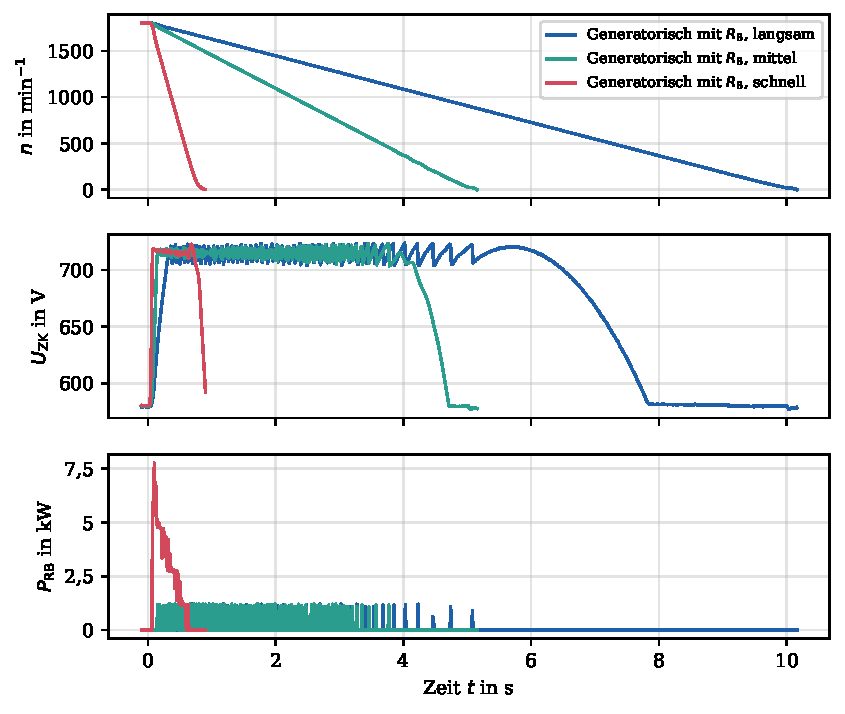
\includegraphics[width=0.72\textwidth]{b_gen}
\end{figure}

\subsection{Bremsmomente im Vergleich}
\begin{figure}[H]\centering
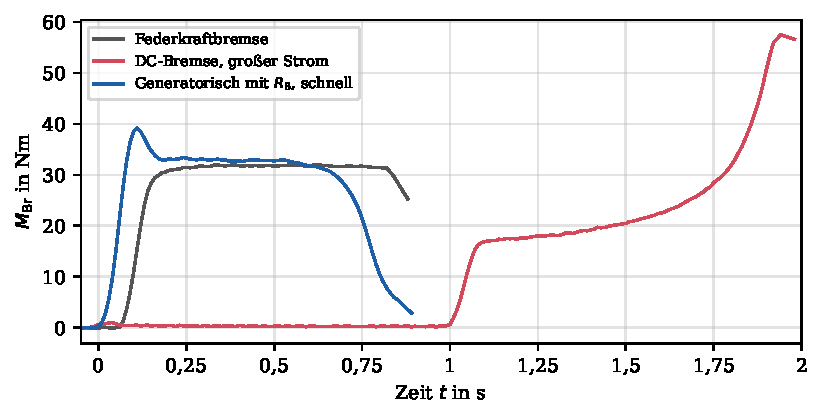
\includegraphics[width=0.8\textwidth]{b_moment_zoom}
\end{figure}
\begin{center}
\begin{tabular}{@{}lccc@{}}
\toprule
Verfahren & Momentverlauf & Haltemoment? & Wo wird die Energie verheizt?\\
\midrule
Federkraftbremse & konstant & ja & Bremsbeläge\\
DC-Bremse & steigt zum Stillstand & nein & Motor (Läufer)\\
Generat.\ ohne $R_B$ & nur kurze Impulse & nein & Verluste, Kondensator\\
Generat.\ mit $R_B$ & konstant (Rampe) & nein & Bremswiderstand\\
\bottomrule
\end{tabular}
\end{center}

% =====================================================================
\section{Die Fragen der Anleitung -- Antworten in eigenen Worten}
% =====================================================================
\begin{frage}{Wodurch entsteht der Spannungseinbruch, und wie kann man ihn verringern?}
\textbf{Ursache:}
\begin{itemize}
\item Der große Anlaufstrom fließt über den Innenwiderstand des Netzes (Trafo und Kabel).
\item Er ist fast reiner Blindstrom, und der Trafo ist vor allem induktiv.
\item Deshalb zieht der Spannungsabfall die Netzspannung direkt nach unten.
\end{itemize}
\textbf{Abhilfe:}
\begin{itemize}
\item Stern-Dreieck (richtig eingestellt), Sanftanlasser, Frequenzumrichter, Anlasstrafo.
\item Größerer Trafo mit kleinem $u_k$, dickere bzw.\ kürzere Kabel.
\end{itemize}
\end{frage}

\begin{frage}{Vergleich berechnete und gemessene Hochlaufzeit}
\begin{itemize}
\item Dreieck: berechnet \SI{\WtHDB}{s}, gemessen \SI{\Wdirektteinsvierfuenfnull}{s}.
\item Stern: berechnet ca.\ \SI{\WtHYum}{s}, gemessen \SI{\Wrichtigtum}{s} (bis \SI{1443}{\per\minute}).
\end{itemize}
Die Messung ist etwas schneller, weil die reale Maschine mehr Moment hat (Toleranz,
\SI{405}{V}, Ablesefehler). Der Verlauf passt sehr gut.
\end{frage}

\begin{frage}{Beschleunigungsmoment berechnen und mit der Vorbereitung vergleichen}
\begin{itemize}
\item Formel: $M = J\cdot2\pi\cdot\mathrm dn/\mathrm dt$ mit $J=\SI{0,3711}{kg.m^2}$.
\item Ergebnis: Die Form gleicht der Kennlinie. Mittelwert im Dreieck \SI{\WdirektMBmittel}{Nm}
      (Kennlinie \SI{\WMkennDmittel}{Nm}), im Stern \SI{\WrichtigMBmittel}{Nm}
      (Kennlinie \SI{\WMkennYmittel}{Nm}).
\end{itemize}
\end{frage}

\begin{frage}{Warum ist generatorisches Bremsen ohne Bremswiderstand so viel langsamer?}
\begin{itemize}
\item Die Energie kann nicht ins Netz zurück, weil der Diodengleichrichter eine Einbahnstraße ist.
\item Ohne Widerstand gibt es keinen Ort, wohin die Energie kann.
\item $U_\mathrm{ZK}$ steigt auf die Überspannungsgrenze, und der FU unterbricht das Bremsen.
\item Mit Widerstand wird die Energie verheizt, und die Rampe wird eingehalten:
      \SI{0,87}{s} statt \SI{8,5}{s}.
\end{itemize}
\end{frage}

\begin{frage}{Welches Verfahren eignet sich als Not-Halt?}
Die \textbf{Federkraftbremse}, weil sie
\begin{itemize}
\item \emph{ohne Strom} bremst (ausfallsicher, Ruhestromprinzip),
\item auch bei Netzausfall und FU-Defekt wirkt,
\item die Last im Stillstand \emph{hält}.
\end{itemize}
Alle elektrischen Verfahren brauchen Netz und FU.
In der Praxis kombiniert man: Zuerst generatorisch bremsen (schont die Beläge), dann fällt die
Federkraftbremse ein (Stopp-Kategorie 1).
\end{frage}

% =====================================================================
\section{Mögliche Testat-Fragen zum Üben}
% =====================================================================
\begin{enumerate}[label=\textbf{F\arabic*:},leftmargin=2.2em]
\item \emph{Warum ist der Anlaufstrom 5- bis 8-mal so groß wie der Nennstrom?}\\
  Bei $s=1$ wirkt der Motor wie ein kurzgeschlossener Trafo, nur die kleine
  Kurzschlussimpedanz begrenzt den Strom.
\item \emph{Warum fällt der Strom erst nach dem Kippmoment stark ab?}\\
  Erst bei kleinem Schlupf wird der Läuferwiderstand $R_2'/s$ groß. Davor bleibt die
  Impedanz klein.
\item \emph{Um welchen Faktor sinken Strom und Moment im Stern?}\\
  Beide auf ein Drittel. Begründung: Strangspannung $/\sqrt3$, $M\sim U^2$, Netzstrom
  $\sqrt3\cdot\sqrt3 = 3$.
\item \emph{Wann darf man keinen Stern-Dreieck-Anlauf verwenden?}\\
  Wenn das Lastmoment beim Anlauf größer als ein Drittel des Motormoments ist, z.\,B.\
  bei schweren Förderbändern oder Hubwerken. Dann besser einen FU verwenden.
\item \emph{Was passiert bei zu frühem Umschalten?}\\
  Ein zweiter Stromstoß, fast wie beim Direktanlauf.
\item \emph{Was passiert bei zu spätem Umschalten oder wenn der Motor im Stern nicht hochkommt?}\\
  Der Motor bleibt bei einer Drehzahl hängen, an der $M_{230} = M_\mathrm{Last}$ ist.
  Er nimmt lange hohen Strom auf und wird thermisch überlastet.
\item \emph{Wie rechnet man aus der Drehzahl das Moment?}\\
  $M = J\cdot 2\pi\cdot \mathrm dn/\mathrm dt$, mit $n$ in \si{\per\second}.
\item \emph{Wie groß ist $J$ einer Vollscheibe?}\\
  $\frac12 m r^2$, Achtung: Radius, nicht Durchmesser!
\item \emph{Warum hat die DC-Bremse kein Haltemoment?}\\
  Ohne Bewegung wird nichts induziert.
\item \emph{Wohin geht die Energie bei der DC-Bremse?}\\
  In den Motor (Läufer und Ständer), er wird heiß.
\item \emph{Warum steigt $U_\mathrm{ZK}$ beim generatorischen Bremsen?}\\
  Energie fließt in den Kondensator, und der Diodengleichrichter kann sie nicht ins Netz abgeben.
\item \emph{Was ist ein Brems-Chopper?}\\
  Ein Transistor, der ab einer Spannungsschwelle den Bremswiderstand an den Zwischenkreis schaltet.
\item \emph{Wie könnte man die Bremsenergie nutzen statt verheizen?}\\
  Mit einem rückspeisefähigen Umrichter (Active Front End) oder mit einem gemeinsamen
  Zwischenkreis mehrerer Antriebe.
\item \emph{Warum ist die Federkraftbremse ausfallsicher?}\\
  Die Feder bremst, der Strom \emph{lüftet} nur. Fällt der Strom aus, wird gebremst.
\item \emph{Warum braucht die DC-Bremse eine Wartezeit vor dem Einspeisen?}\\
  Der Motor ist noch magnetisiert und erzeugt eine Restspannung. Würde der FU sofort
  einspeisen, gäbe es Überströme.
\end{enumerate}

% =====================================================================
\section{Formelsammlung auf einen Blick}
% =====================================================================
\begin{center}
\renewcommand{\arraystretch}{1.5}
\begin{tabular}{@{}ll@{}}
\toprule
Synchrondrehzahl & $n_s = f/p$\\
Schlupf & $s = (n_s - n)/n_s$\\
Leistung -- Moment & $P = M\cdot\omega = M\cdot 2\pi n$\\
Moment und Spannung & $M \sim U^2$, \quad $M_{230} = \frac13 M_{400}$\\
Bewegungsgleichung & $J\,\mathrm d\omega/\mathrm dt = M_\mathrm{Mot} - M_\mathrm{Last}$\\
Zeitschritt & $\Delta t = 2\pi J \Delta n / M$\\
Trägheitsmoment Vollscheibe & $J = \frac12 m r^2$\\
kinetische Energie & $E = \frac12 J\omega^2$\\
Spannungsabfall (Kapp) & $\Delta U \approx I(R_k\cos\varphi + X_k\sin\varphi)$\\
Leistungsfaktor & $\cos\varphi = P/\sqrt{P^2+Q^2}$\\
DC-Bremsmoment & $M_\mathrm{Br} \sim I_\mathrm{DC}^2$\\
\bottomrule
\end{tabular}
\end{center}

% =====================================================================
\section{Wichtige Hinweise zu deinen Dateien}
% =====================================================================
\begin{itemize}
\item \textbf{Nicht verwendet:} Die Dateien \texttt{F\_Kennline\_Dreick.csv},
  \texttt{F\_Kennline\_Stern.csv} und \texttt{Messung\_f87Hz\_*.csv} gehören nicht zu V9.
  Sie sind Frequenzkennlinien bzw.\ ein 87-Hz-Betrieb und stammen vermutlich aus einem
  anderen Versuch. Deshalb sind sie nicht im Bericht.
\item \textbf{Namen der Dateien:} \texttt{Stern-Dreieck\_direkt.csv} ist der
  \emph{direkte Dreieckanlauf} (das sieht man am Anlaufstrom von \SI{50}{A}).
\item \textbf{Vor der Abgabe ausfüllen:} Deckblatt (Namen, Matrikelnummern, Gruppe, Datum).
  Prüfe auch die Umschaltzeit „zu früh“ (\SI{0,5}{s} laut Anleitung, \SI{1,9}{s} in den Daten).
\item \textbf{Ändern:} Wenn du Zahlen ändern willst, ändere die Daten oder das Skript
  \texttt{auswertung/auswertung.py}, führe es aus (\texttt{python3 auswertung.py}) und
  übersetze den Bericht neu. Alle Zahlen im Text aktualisieren sich dann automatisch.
\end{itemize}
\end{document}
